\footnotesize

\section{Introduction}

	\begin{frame}
		\begin{center}
			\LARGE{Introduction}
		\end{center}
	\end{frame}

	\subsection{General Introduction}
		
		\begin{frame}
			\frametitle{Introduction}	
			\begin{block}{Generals}
				\begin{itemize}\vspace{0.3cm}
					\item The IEEE 42010 standard is an international standard for architecture description of \emph{systems} and \emph{software}\vspace{0.3cm}
					\item It addresses the creation, analysis and sustainment of architectures through the use of \emph{architecture description}\vspace{0.3cm}
					\item It is an evolution of the IEEE 1471:2000 standard. The main concepts are generalized in order to address a huge variety of systems\vspace{0.3cm}
				\end{itemize}
			\end{block}					
		\end{frame}
	
	\subsection{Standard Introduction}	
	
		\begin{frame}
		\frametitle{Introduction}	
			\begin{block}{What does the standard do?}
			\vspace{0.3cm}
				\begin{itemize}\vspace{0.3cm}
					\item The standard defines a formal conceptual model of Architecture Description\vspace{0.3cm}
					\item It specifies the required contents of an Architecture Description\vspace{0.3cm}
					\item Architecture viewpoints, frameworks and description languages are introduced and the contents of these are specified\vspace{0.3cm}
					\item It also provides motivation and background for \emph{key concepts} and \emph{terminology} of the standard\vspace{0.3cm}
				\end{itemize}			
			\end{block}
		\end{frame}
		
		\begin{frame}
		\vspace{0.3cm}
			The ISO/IEC/IEEE 42010:2011 standard consists of several parts, each one addressing different issues about the definition of a system and the description of its architecture.
			\newline\newline
			
			These parts define a standard set of terms used to define architecture descriptions, guidelines for the metamodel that has to be done and a set of "best practices" for the description and the requirement definition of the system.
			\newline\newline
			
		We will focus on the first two parts of the standard, which are of uttermost interest for our job.
		
		\end{frame}
		
		\subsection{Elements of the Standard}
		
		\begin{frame}
			
		\vspace{0.3cm}
		
			\begin{block}{Conceptual Model}
				\begin{itemize}
					\item The \emph{conceptual model} of architecture descriptions (also called "metamodel") define the set of terms, their definitions and the relations among them. These are then used in expressing the requirements of the system
				\end{itemize}
			\end{block}				
			
\vspace{0.3cm}			
			
			\begin{block}{Architecture Description}
				\begin{itemize}
					\item The standard defines \emph{architecture descriptions} as a way to express an Architecture and specifies the requirements the architecture descriptions have to meet in order to satisfy the standard. However, it does not define what \emph{form} has to be used to provide the description (i.e. it can be a document, a repository, a wiki\dots)
				\end{itemize}
			\end{block}
		\end{frame}
		
		\begin{frame}					
			
			\begin{block}{Architecture Viewpoints}
			\begin{itemize}
				\item At the core of the standard there is the idea of \emph{architecture viewpoints}. A viewpoint is a way of looking at the architecture of a system. Viewpoints are strongly related with the level of detail required to model a certain view (e.g. cyber-physical, informative, service level)
				\end{itemize}
			\end{block}
				
			\begin{block}{Architecture Frameworks and ADLs}
				\begin{itemize}
					\item The last section of the standard specifies \emph{best practices} for \emph{architecture frameworks}.\newline
					The focus is on the specification of the best practices for documenting the architecture of a system. As we know, documentation has to be used for the \emph{whole} lifetime of a system (starting from its design to its implementation).\newline
					The principles used with architecture frameworks can be used in a similar manner with ADLs (Architecture Description Languages)
				\end{itemize}
			
			\end{block}
		\end{frame}
		
\section{Description of the Standard}

	\begin{frame}
		\begin{LARGE}
			Conformance to ISO/IEC/IEEE 42010:2011
		\end{LARGE}
	\end{frame}
	
	\subsection{Introduction}
	
		\begin{frame}
			\vspace{0.3cm}
			In the previous section we had an overview of the standard, what is its focus and what are main parts it consists of.\newline\newline
			In this section we will have a deeper look at the definition of the conceptual model and some of the requirements an architecture has to meet in order to conform to the standard, that is: an explanation of what is an \emph{Architecture Description} along with the requirements it has to meet and what is the role of the conceptual model.\newline\newline
			In the end we will see the process that must be followed in order to create a "sound" Architecture Description and how to determine Architecture Viewpoints.
		\end{frame}
		
	\subsection{Conceptual Model}
	
		\begin{frame}
			\begin{block}{Conceptual Model}
			\vspace{0.2cm}
				\begin{itemize}
				\item The standard itself is based upon a conceptual model of the terms and concepts pertaining to \emph{Architecture Description}
				\item This metamodel guides the system (or software) designer in the process of creating an Architecture Description
				\item It is divided in different section, each addressing different problems and/or perspectives of the architecture
					\begin{itemize}
						\item[1.] Context
						\item[2.] Core of Architecture Description
						\item[3.] AD Elements and Correspondences
						\item[4.] Architecture Decisions and Rationale
						\item[5.] Architecture Frameworks and ADLs
					\end{itemize}
				\end{itemize}
				\vspace{0.2cm}
			\end{block}
		\end{frame}
		
		\begin{frame}
			\begin{block}{Conceptual Model Overview}
				\begin{itemize}
					\item The "Context" diagram captures terms and concepts of systems and their architectures. These are used as a \emph{Context} for understanding Architecture Description
					\item The standard is organized around terms and concepts introduced in the Architecture Description diagram. This diagram depicts the contents of an AD and the relations among those items to produce an \emph{Architecture Description} to express an \emph{Architecture} for the \emph{System of Interest}
					\item ADs are comprised of \emph{AD elements}. \emph{Corrispondences} and \emph{Corrispondence Rules} capture and express relathionships between these elements
					\item \emph{Architecture Decisions} and \emph{Rationales} are used to keep a trace of architecture decisions made during the design of the architecture (such as conventions, technologies involved, design decisions)
					\item \emph{Architecture Frameworks} and \emph{ADLs} can be easily specified by building on the concepts of \emph{Architecture Description}
				\end{itemize}
			\end{block}
		\end{frame}
		
		\begin{frame}
			\begin{center}
				\begin{LARGE}
					CONTEXT
				\end{LARGE}
			\end{center}
		\end{frame}
		
		\begin{frame}
					\begin{figure}
						\begin{center}
							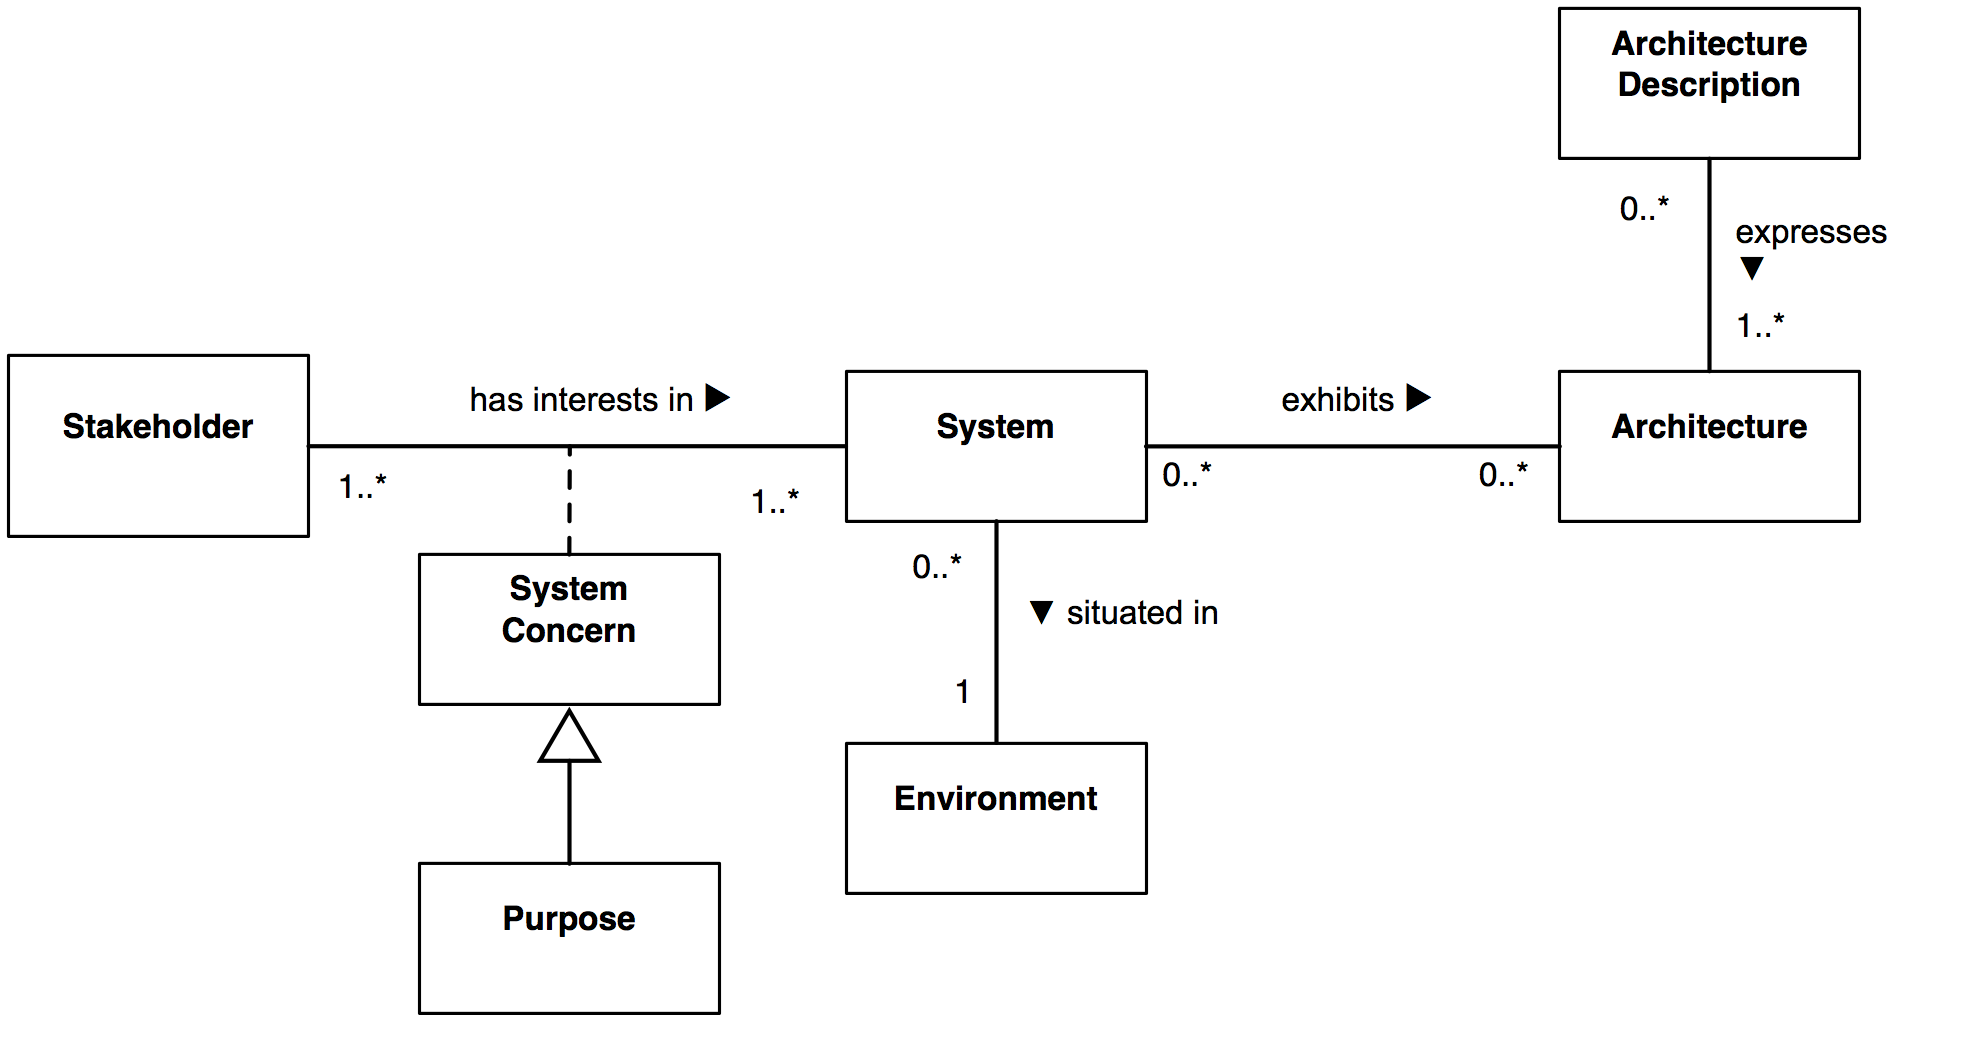
\includegraphics[width=\textwidth]{img/ConceptualModelContext}
						\end{center}
					\end{figure}
		\end{frame}
		
		\begin{frame}
			\begin{itemize}
				\item The diagram assumes that a system exists, it is situated in an \emph{Environment} that could include other systems.
				\item The standard does not make any assumption on the kind of the system. This means it can be either a system, a SoS, Physical system (man-made or natural)\dots
				\item Stakeholders have interests in a System. These interests are called \emph{Concerns}. A system's \emph{Purpose} is a Concern that is common to (possibly) all the Stakeholders.
				\item A system inhabits its \emph{Environment}. The system influences the Environment and vice versa. The Environment of a system determines all the influences upon the system. These influences are categorized as Concerns.
				\item In the standard, the \emph{architecture} of a system has a formal definition, that is: “fundamental concepts or properties of a system in its environment embodied in its elements, relationships, and in the principles of its design and evolution”.
				\item An \emph{Architecture Description} is an artifact that expresses the system's architecture.
			\end{itemize}
		\end{frame}
		
		\begin{frame}
		\begin{center}
				\begin{LARGE}
					ARCHITECTURE DESCRIPTION
				\end{LARGE}
			\end{center}
		\end{frame}
		
		\begin{frame}
					\begin{figure}
						\begin{center}
							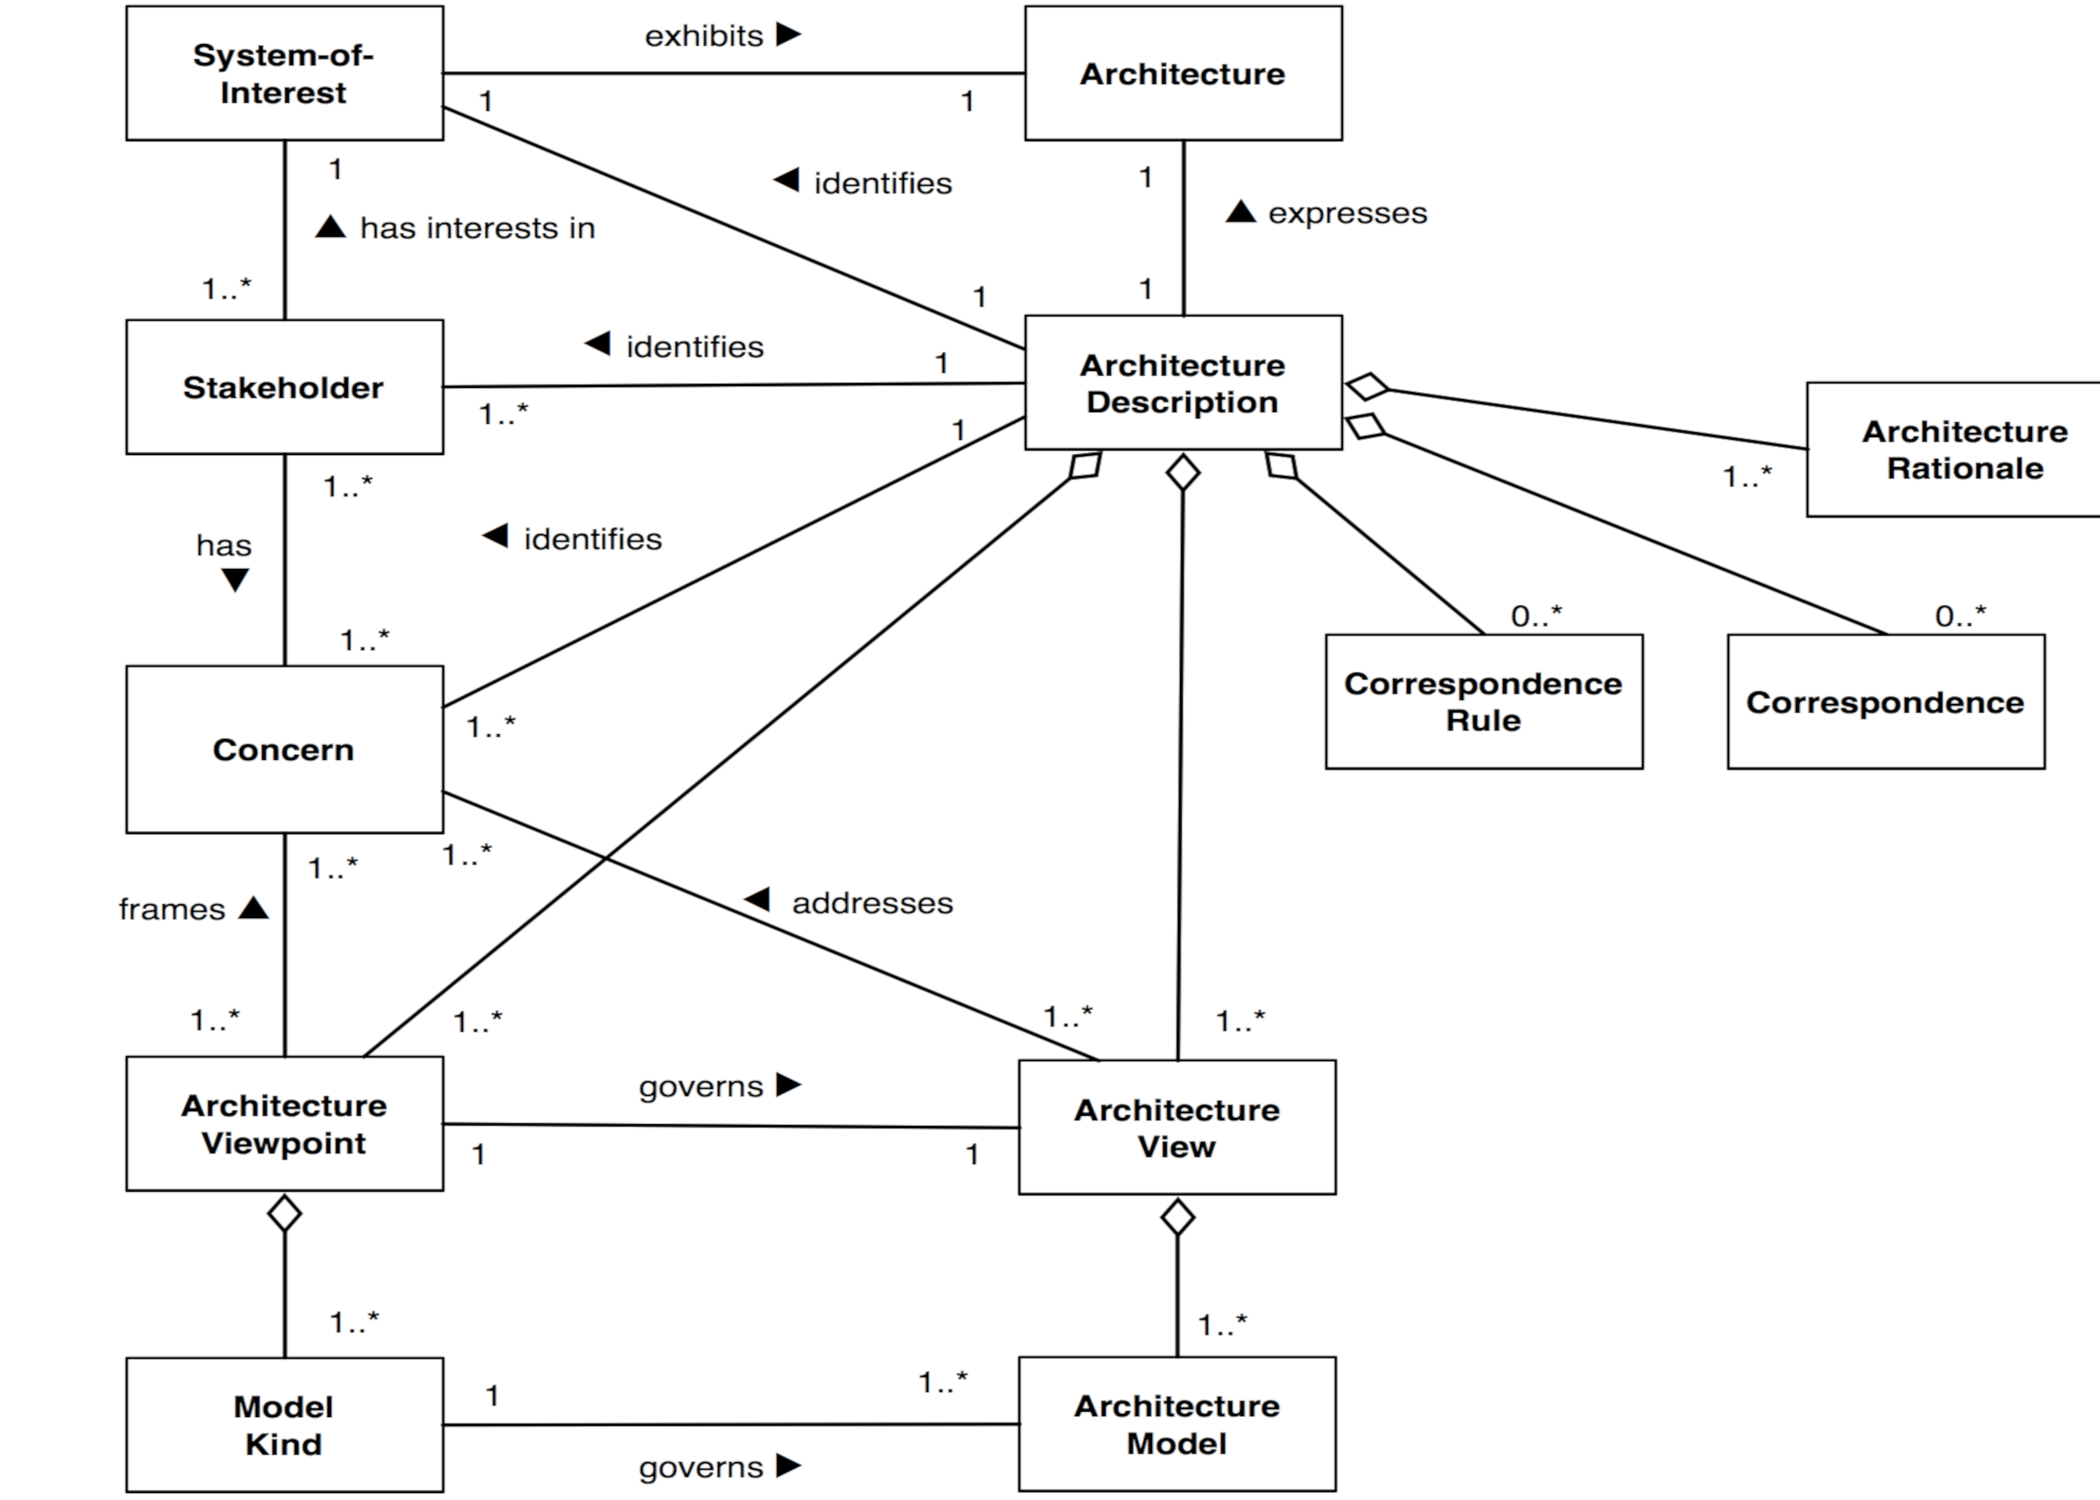
\includegraphics[width=\textwidth]{img/ConceptualModelArchitectureDescription}
						\end{center}
					\end{figure}
		\end{frame}
		
		\begin{frame}
			\begin{itemize}
				\item An \emph{Architecture Description} is used to express the Architecture of some System of Interest. The AD describes one possible Architecture for the System of Interest whose requirements are specified by the standard.
				\item \emph{Stakeholders} are individuals, groups or organizations holding Concerns for the System (e.g. client, owner, consumer, designer\dots)
				\item A \emph{Concern} is \textbf{any interest} in the system (i.e. system purpose, functionality, structure, behaviour, \emph{safety}\dots)
				\item An \emph{Architecture Viewpoint} is a set of conventions for constructing, using and analyzing \textbf{one} type of Architecture View and it includes Model kinds, notations, modeling methods and analytic techniques to frame a \emph{specific set of Concerns}. Examples of Viewpoints are: operational, technical, logical, information\dots
				\item An \emph{Architecture View} in an AD expresses the Architecture of the System from the perspective of the Stakeholders to address specific Concerns and it consists of one or more Architecture Models
				\item \emph{Architecture Models} are constructed in accordance with the conventions established in their Model Kind. Models provide means for sharing details among different views
				\item A \emph{Model Kind} defines the conventions for \textbf{one} type of Architecture Model
			\end{itemize}
		\end{frame}
		
	\begin{frame}
		\begin{center}
				\begin{LARGE}
					ARCHITECTURE DESCRIPTION\newline\newline ELEMENTS AND CORRESPONDENCES
				\end{LARGE}
			\end{center}
		\end{frame}
		
		\begin{frame}
					\begin{figure}
						\begin{center}
							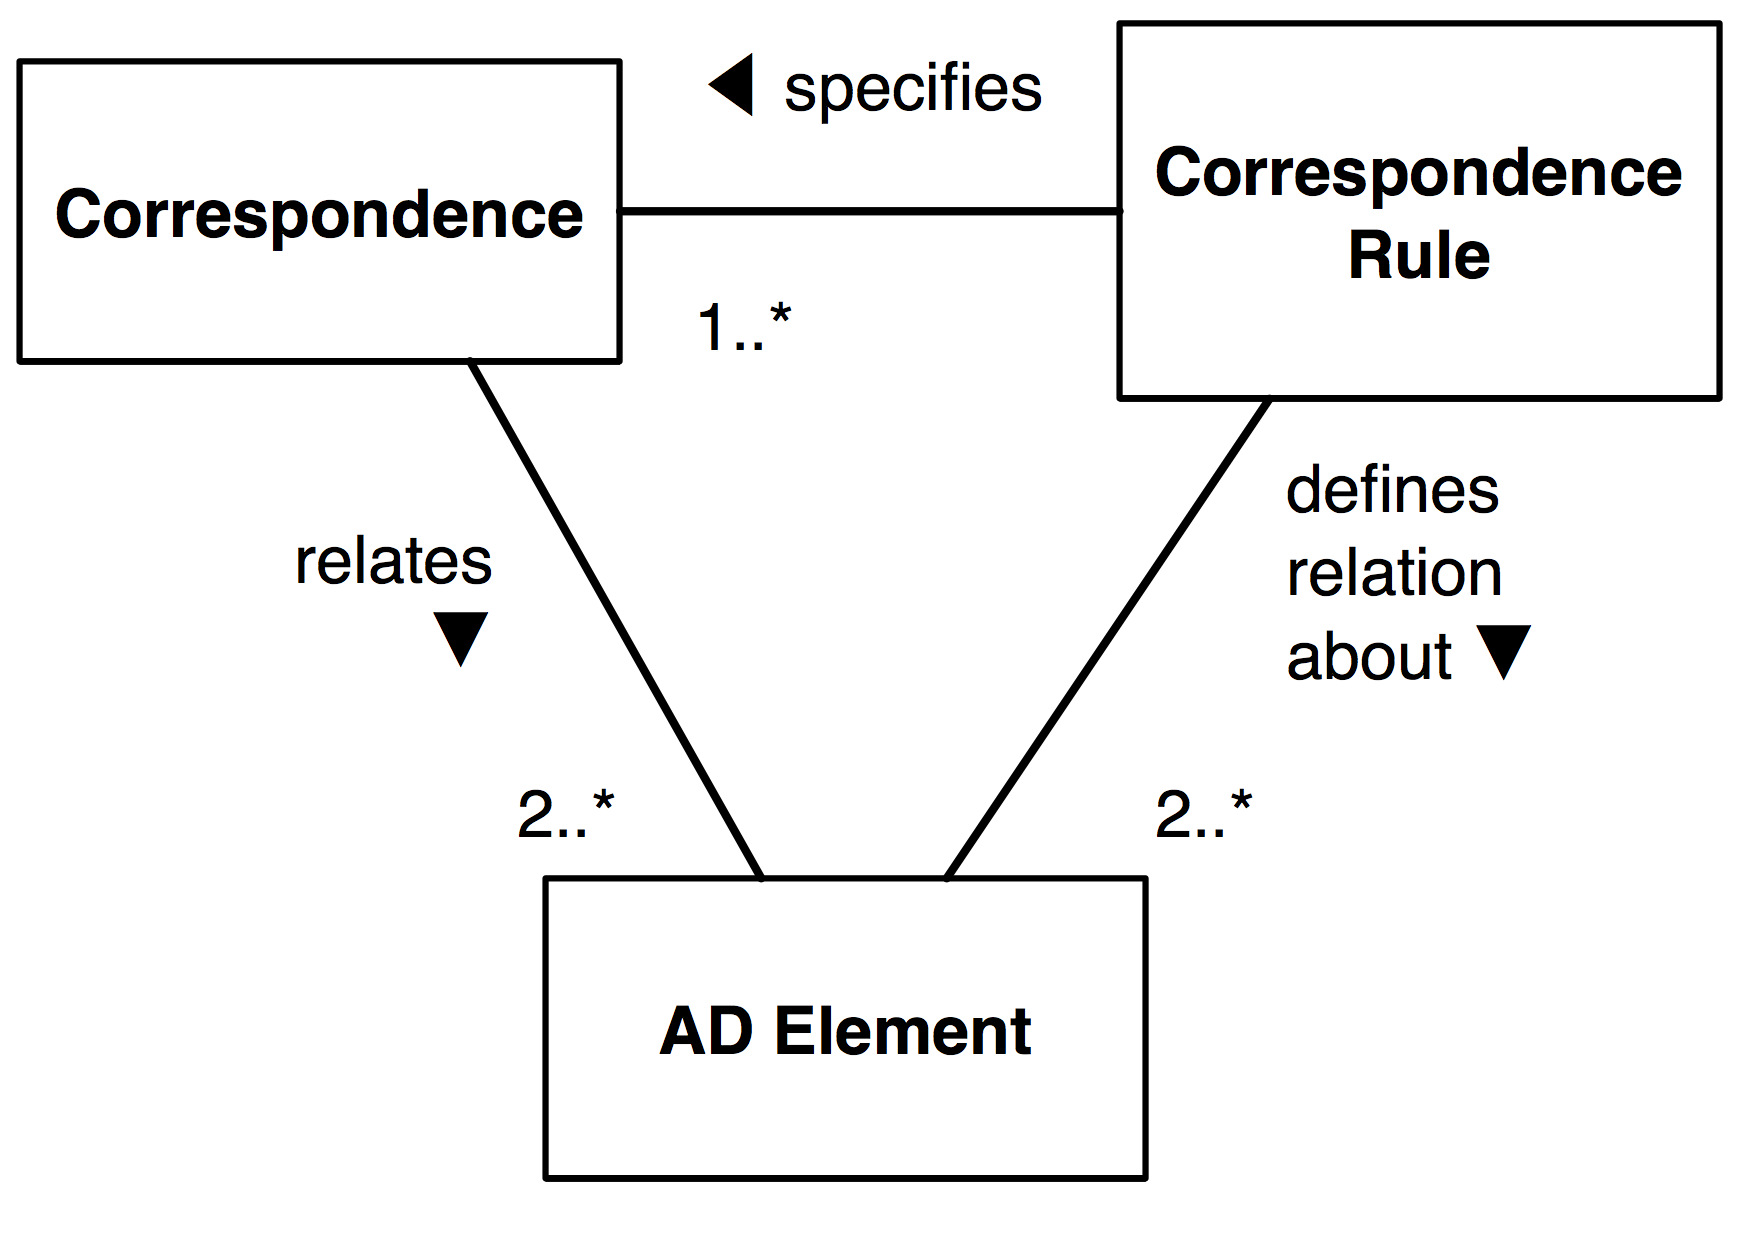
\includegraphics[width=\textwidth]{img/ConceptualModelArchitectureDescriptionElements}
						\end{center}
					\end{figure}
		\end{frame}
		
		\begin{frame}
			\begin{itemize}
				\item Any item in an AD is considered an \emph{AD Element}. Stakeholders, Concerns, Viewpoints etc. are all AD Elements, as well as constructs introduced by Viewpoints or Model Kinds
				\vspace{0.3cm}
				\item \emph{Correspondences} express relations between AD Elements. They can also describe relations between two different ADs
				\vspace{0.3cm}
				\item \emph{Correspondence Rules} are used to govern Correspondences
			\end{itemize}
		\end{frame}
		
			\begin{frame}
		\begin{center}
				\begin{LARGE}
					ARCHITECTURE DECISIONS\newline\newline AND RATIONALE
				\end{LARGE}
			\end{center}
		\end{frame}
		
		\begin{frame}
					\begin{figure}
						\begin{center}
							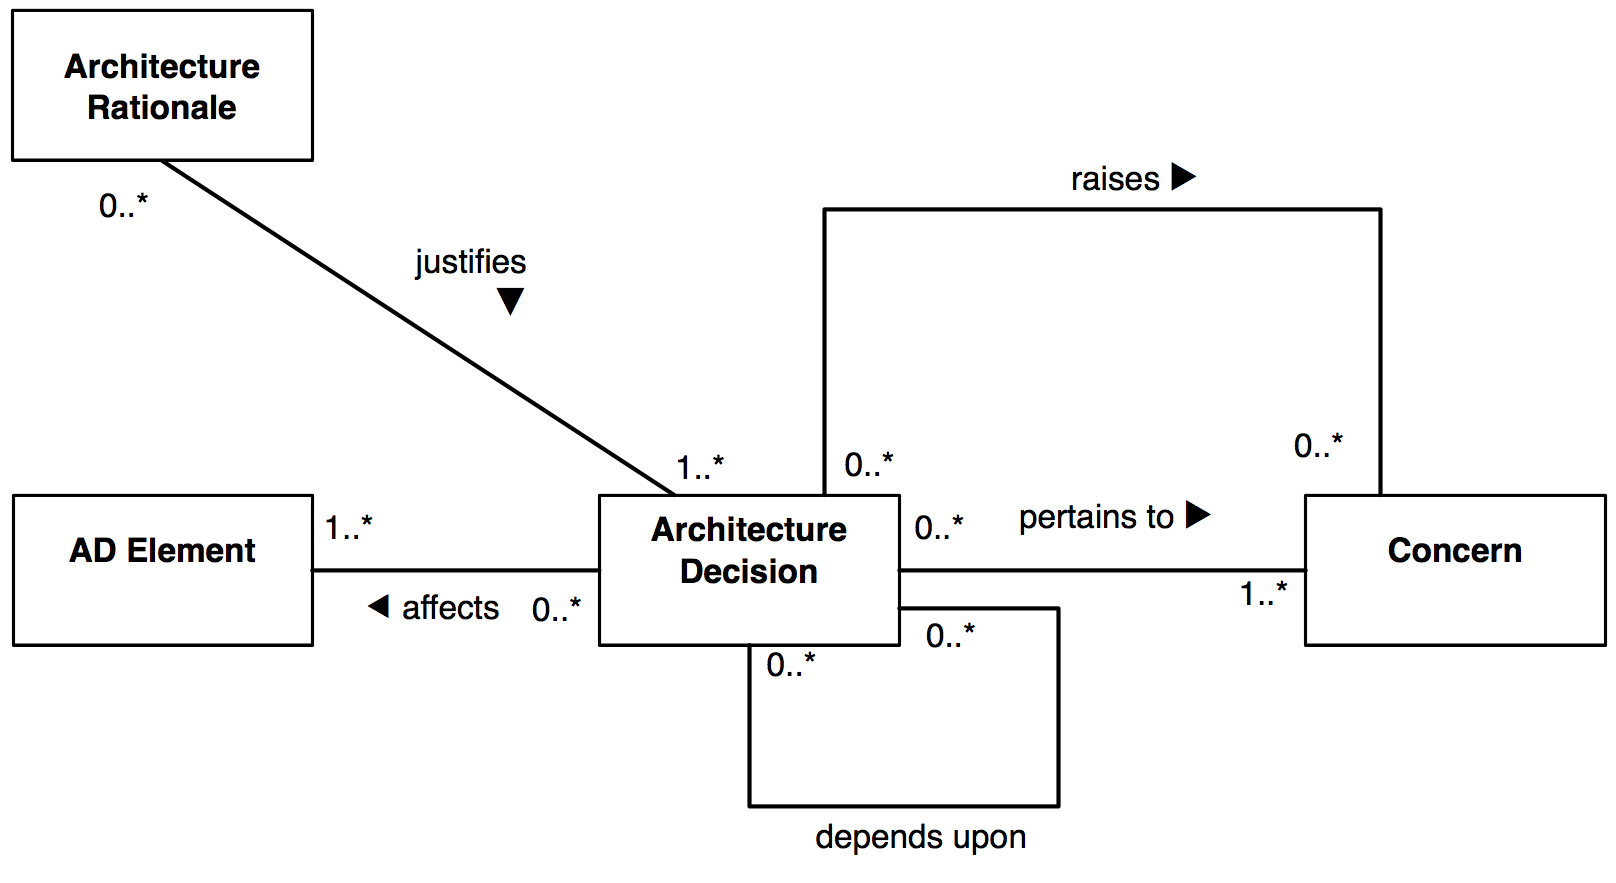
\includegraphics[width=\textwidth]{img/ConceptualModelRationale}
						\end{center}
					\end{figure}
		\end{frame}
		
		\begin{frame}
			\begin{itemize}
				\item \emph{Architecture Decisions} affects AD Elements and pertains to one or more Concerns. Architecture Decisions could raise new Concerns.
				\vspace{0.3cm}
				\item \emph{Architecture Rationale} is used to record explanation, justification or reasoning about Architecture Decisions and/or architectural alternatives not chosen
			\end{itemize}
		\end{frame}
		
		\begin{frame}
		\begin{center}
				\begin{LARGE}
					ARCHITECTURE FRAMEWORKS\newline\newline AND ADLs
				\end{LARGE}
			\end{center}
		\end{frame}
		
		\begin{frame}
					\begin{figure}
						\begin{center}
							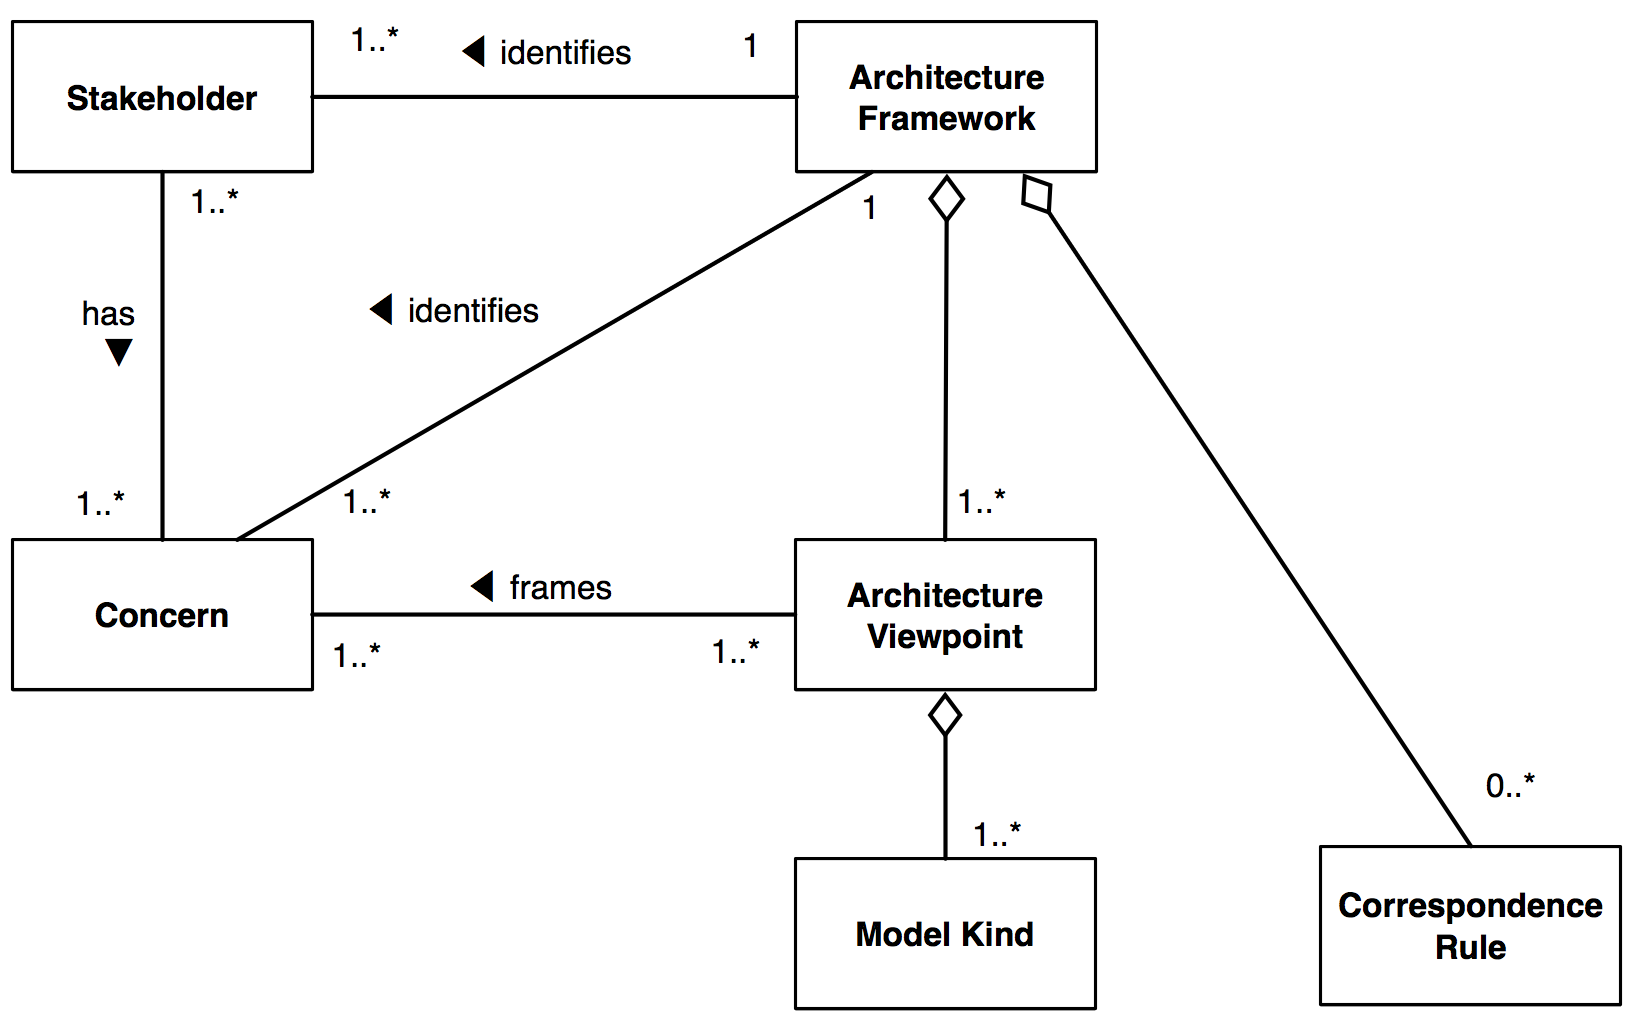
\includegraphics[width=\textwidth]{img/ConceptualModelFramework}
						\end{center}
					\end{figure}
		\end{frame}
		
		\begin{frame}
			\begin{figure}
						\begin{center}
							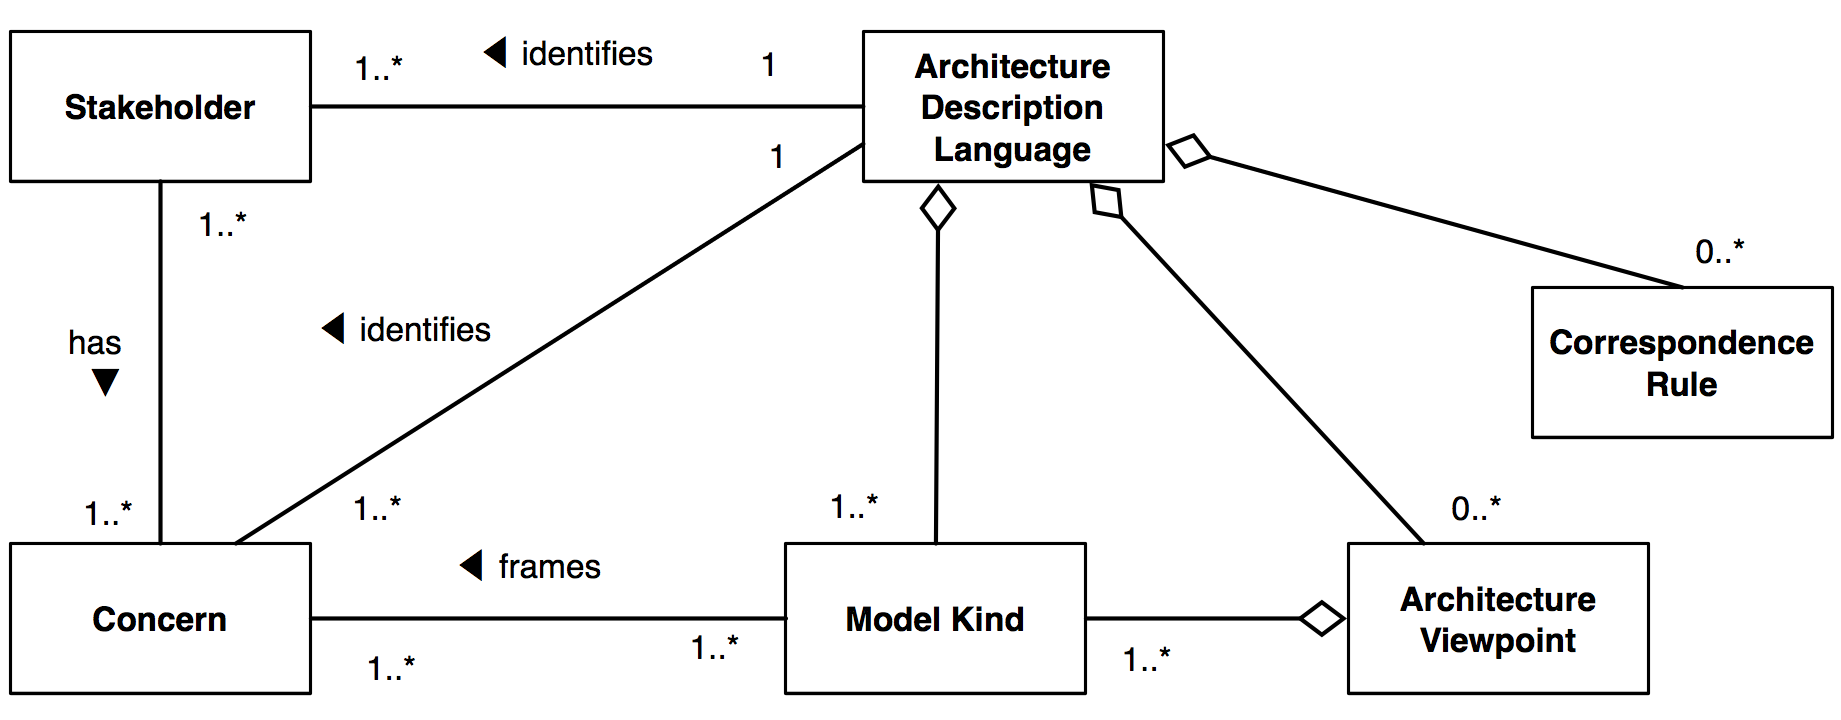
\includegraphics[width=\textwidth]{img/ConceptualModelADL}
						\end{center}
					\end{figure}
		\end{frame}
		
		\subsection{Architecture Description and Viewpoints}
		
		\begin{frame}
			\begin{center}
				\begin{LARGE}
					ARCHITECTURE DESCRIPTION\newline\newline AND VIEWPOINTS
				\end{LARGE}
			\end{center}
		\end{frame}
				
		
		\begin{frame}
		
		At this point, we had an overview of the standard, along with its main concepts and the established Conceptual Model used to guide us in the creation of the System.
		\newline\newline
		
		After all this, it's useful to have a quick look at how the standard defines \emph{Architecture Descriptions} and \emph{Architecture Viewpoints}, that are at the core of it.\newline\newline
		
		In this section we will see the process for preparing an AD and how the Architecture Viewpoints are determined.
		
		\end{frame}
		
		\begin{frame}
			\begin{block}{Architecture Description}
				\begin{itemize}
				\vspace{0.3cm}
					\item An Architecture Description identifies the System-of-interest and expresses its Architecture
					\vspace{0.3cm}
					\item The central part of the standard describes the best practices for creating an AD
\vspace{0.3cm}				
					\item It is a list of 24 requirements ("shalls")
\vspace{0.3cm}				
					\item An AD \emph{conforms} to the Standard if it satisfies all the requirements
\vspace{0.3cm}					
					\item The Standard does not make any assumption on what kind of System we are going to describe, nor the \emph{form} of the description
					\vspace{0.3cm}
					\item The Standard gives Templates in order to facilitate the process of creation of the AD
					\vspace{0.3cm}
				\end{itemize}
			\end{block}
		\end{frame}				
		
		\begin{frame}
		Taken together, the list of requirements expressed by the Standard gives us a process for creating the AD:
			\begin{block}{Architecture Description Process}
			\begin{itemize}
				\item[1.] Identification of the relevant Stakeholders and record them in the AD
				\item[2.] Identification of the Architecture Concerns of each Stakeholder:
					\begin{itemize}
						\item Purposes of the System
						\item Suitability of the Architecture for achieving System's purposes
						\item Feasibility of constructing the System
						\item Potential risks and impacts of the System to its Stakeholders, throughout the whole life-cycle
						\item Maintainability and Evolvability of the System
					\end{itemize}
				\item[3.] Choose one (or more) Architecture Viewpoints for expressing the Architecture such that \emph{each} Concern is \emph{framed} by at least one Viewpoint
				\item[4.] Record those Viewpoints in the AD and provide a \emph{Rationale} for each choice of Viewpoint 
			\end{itemize}
			\end{block}
			
		\end{frame}
		
		\begin{frame}
			\begin{block}{Architecture Description Process}
				\begin{itemize}
					\item[5.] Document each Viewpoint with a \emph{Viewpoint Definition}. Each Viewpoint Definition links the Stakeholders and Concerns to the kinds of notation and model to be used
					\item[6.] Create Architecture Views of the System, for each chosen Viewpoint, following the conventions of its Viewpoint. Views must include:
						\begin{itemize}
							\item One, or more, models
							\item Identifying informations
						\end{itemize}
					\item[7.] Document correspondences between Views and Model Elements, guarantee consistency across views, record inconsistencies
					\item[8.] Record the AD Rationales for architecture decisions and \emph{give evidence of the consideration of multiple architectures}
				\end{itemize}
			\end{block}
		\end{frame}
		
		\begin{frame}
			We understand that ADs are characterized by the different Viewpoints we can choose to describe it.\newline\newline
			But how are Viewpoints determined? The Standard gives us a guideline for this too:
			\begin{block}{Determining Viewpoints}
				An Architecture Viewpoint is determined by:
				\begin{itemize}
					\item One or more concerns
					\item Stakeholders interested in those concerns (which constitute a potential audience for views resulting from this viewpoint)
					\item One or more Model Kinds
					\item For each Model Kind, the conventions, such as: languages, notations, modelling and analytical techniques\dots
				\end{itemize}
			\end{block}
		\end{frame}				
		
		\section{Conclusion}
		
		\begin{frame}
			\begin{itemize}
			
			\item The ISO/IEC/IEEE 42010:2011 standard sets its focus on documenting an Architecture
			
			\vspace{0.3cm}
			\item It is also useful to address \textbf{every} aspect of interest in the System to be made
			
			\vspace{0.3cm}
			\item The standard does not make any assumption on what kind of System we are about to document, keeping its definition the most general it can, allowing to describe any kind of system (either physical or cyber)
			\vspace{0.3cm}
			\item In this way we are able to observe every aspect of the System we have to study, to maintain a trace of design choices and it helps us to address every element that could have an impact on it
			\end{itemize}
		\end{frame}
		
		\begin{frame}
			\begin{LARGE}
			\begin{center}
			
				THANKS FOR YOUR ATTENTION

			\end{center}			
			\end{LARGE}
			\begin{figure}
						\begin{center}
							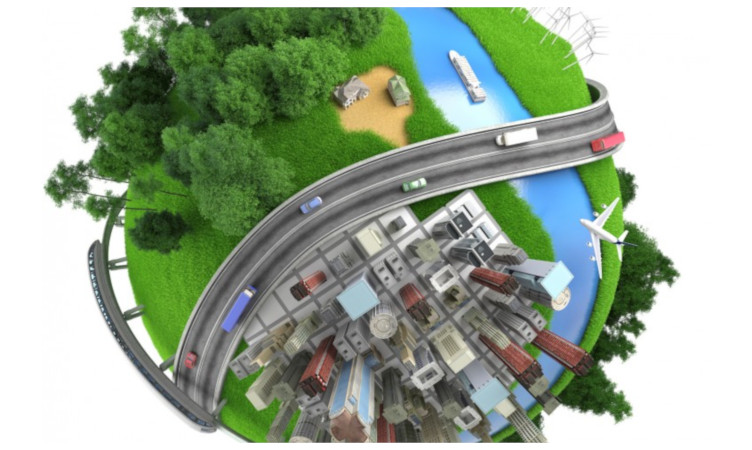
\includegraphics[width=\textwidth]{img/system-of-systems}
						\end{center}
					\end{figure}
		\end{frame}
		
		\section{Bibliography}
		
		\begin{frame}
			\begin{block}{References}
			
			\begin{itemize}
			\vspace{0.3cm}
				\item \url{http://www.iso-architecture.org/ieee-1471/getting-started.html}
			\vspace{0.3cm}
				\item \url{http://www.iso-architecture.org/ieee-1471/cm/}
			\vspace{0.3cm}
				\item \url{http://www.iso-architecture.org/ieee-1471/ads/}
			\vspace{0.3cm}
				\item \url{https://en.wikipedia.org/wiki/ISO/IEC_42010}
			\vspace{0.3cm}
			\end{itemize}

			\end{block}		
		\end{frame}